\appendix
\chapter{Результаты тематического моделирования} \label{app:topics}
\textbf{0. Детская медицина}

0.040*ребёнок + 0.020*больница + 0.019*девочка + 0.019*омск + 0.016*мальчик + 0.012*медицинский + 0.012*врач + 0.010*область + 0.009*женщина + 0.009*находиться + 0.009*помощь + 0.008*мать + 0.008*полиция + 0.007*родитель + 0.007*подросток + 0.007*состояние + 0.007*сообщить + 0.006*время + 0.006*проверка + 0.006*дом

\textbf{1. Местная власть}

0.034*омск + 0.028*губернатор + 0.026*назаров + 0.020*виктор + 0.018*область + 0.015*глава + 0.014*регион + 0.010*мэр + 0.008*вячеслав + 0.008*двораковский + 0.008*министр + 0.008*правительство + 0.007*сегодня + 0.007*вопрос + 0.007*россия + 0.006*заявить + 0.006*первый + 0.005*синюгин + 0.005*развитие + 0.005*президент

\textbf{\underline{2. Сложно определить}}

0.009*человек + 0.007*большой + 0.006*нужно + 0.005*город + 0.005*омск + 0.005*время + 0.005*деньги + 0.005*сделать + 0.004*хороший + 0.004*вопрос + 0.004*делать + 0.004*знать + 0.004*проблема + 0.004*журналист + 0.004*работа + 0.004*работать + 0.004*должный + 0.003*проект + 0.003*метро + 0.003*думать

\textbf{3. IT}

0.013*система + 0.009*новый + 0.009*сайт + 0.009*сеть + 0.008*интернет + 0.008*связь + 0.007*мобильный + 0.006*информация + 0.006*оператор + 0.006*россия + 0.006*пользователь + 0.006*компания + 0.006*электронный + 0.006*tele2 + 0.006*услуга + 0.005*абонент + 0.005*время + 0.005*доступ + 0.004*космический + 0.004*дать

\textbf{4. Пожары}

0.024*пожар + 0.022*омск + 0.016*дом + 0.015*человек + 0.013*мчс + 0.012*пожарный + 0.010*область + 0.009*произойти + 0.009*место + 0.009*улица + 0.008*причина + 0.008*сообщить + 0.007*часы + 0.007*огонь + 0.007*результат + 0.006*сообщение + 0.006*мужчина + 0.006*сегодня + 0.006*происшествие + 0.006*возгорание

\textbf{\underline{5. Сложно определить}}

0.025*омск + 0.012*область + 0.011*рейтинг + 0.011*компания + 0.009*омич + 0.009*место + 0.008*тариф + 0.007*регион + 0.007*оао + 0.007*город + 0.007*население + 0.006*сибирь + 0.006*житель + 0.006*2013 + 0.006*число + 0.006*рэк + 0.005*показатель + 0.005*тысяча + 0.005*россия + 0.005*уровень

\textbf{6. Деятельность правоохранительных органов}

0.030*омск + 0.018*россия + 0.015*полиция + 0.015*сотрудник + 0.012*область + 0.012*полицейский + 0.010*умвд + 0.007*гражданин + 0.007*проверка + 0.007*задержать + 0.006*пресс-служба + 0.006*наркотик + 0.006*алкоголь + 0.006*территория + 0.005*обнаружить + 0.005*изъять + 0.005*омич + 0.005*дело + 0.005*административный + 0.005*сообщить

\textbf{7. Экономика области}

0.030*омск + 0.016*область + 0.012*предприятие + 0.011*регион + 0.010*развитие + 0.009*производство + 0.009*продукция + 0.008*проект + 0.007*завод + 0.007*компания + 0.006*продукт + 0.005*россия + 0.005*рынок + 0.005*бизнес + 0.004*новый + 0.004*цена + 0.004*предприниматель + 0.004*хозяйство + 0.004*комплекс + 0.004*реализация

\textbf{8. Банковский сектор}

0.024*компания + 0.020*банка + 0.019*клиент + 0.019*магазин + 0.017*банк + 0.013*кредит + 0.010*карта + 0.008*новый + 0.007*покупка + 0.007*услуга + 0.007*рубль + 0.007*кредитный + 0.006*салон + 0.006*россия + 0.006*банковский + 0.006*продажа + 0.006*сеть + 0.006*товар + 0.006*плюс + 0.006*покупатель

\textbf{9. Праздники, свадьбы}

0.010*день + 0.007*праздник + 0.006*подарок + 0.005*... + 0.004*хороший + 0.004*большой + 0.004*костюм + 0.004*девушка + 0.004*кольцо + 0.004*друг + 0.004*время + 0.004*пара + 0.004*земля + 0.003*цвета + 0.003*новый + 0.003*сделать + 0.003*женщина + 0.003*гость + 0.003*зоопарк + 0.003*брак

\textbf{10. Суды}

0.026*суд + 0.019*омск + 0.016*рубль + 0.015*прокуратура + 0.014*тысяча + 0.011*нарушение + 0.008*область + 0.007*проверка + 0.007*дело + 0.007*штраф + 0.007*требование + 0.006*закон + 0.006*россия + 0.006*признать + 0.006*решение + 0.006*прокурор + 0.006*размер + 0.006*лицо + 0.006*районный + 0.005*срок

\textbf{11. Организация движения и общественный транспорт}

0.069*улица + 0.024*транспорт + 0.020*движение + 0.019*маршрут + 0.019*автобус + 0.016*омск + 0.010*№ + 0.010*проспект + 0.009*пробка + 0.009*маркс + 0.008*участок + 0.008*часы + 0.007*город + 0.007*департамент + 0.007*остановка + 0.006*транспортный + 0.006*ленин + 0.005*путь + 0.005*работа + 0.005*поворот

\textbf{12. Погода}

0.030*омск + 0.018*температура + 0.017*день + 0.015*снег + 0.014*погода + 0.014*воздух + 0.012*градус + 0.011*ветер + 0.010*область + 0.010*днём + 0.009*ожидаться + 0.009*дождь + 0.008*ночью + 0.007*выходной + 0.006*составить + 0.006*неделя + 0.006*управление + 0.006*м/с + 0.005*атмосферный + 0.005*тёплый

\textbf{13. Дело Юрия Гамбурга\footnotemark}\footnotetext{Бывший вице-мэр города Омска. Арестован по обвинению в коррупции.}

0.028*гамбург + 0.014*юрий + 0.014*военный + 0.010*суд + 0.009*пенсионный + 0.007*адвокат + 0.007*пенсия + 0.006*дело + 0.006*часть + 0.006*отношение + 0.006*министр + 0.006*имущественный + 0.006*вице-губернатор + 0.005*следствие + 0.005*первое + 0.005*меренкова + 0.005*решение + 0.005*арест + 0.005*оборона + 0.005*находиться

\textbf{14. Военные учения}

0.016*учение + 0.016*ракета + 0.015*корабль + 0.012*вопрос + 0.011*чёрный + 0.010*мор + 0.009*море + 0.008*ракетный + 0.007*ответ + 0.007*полигон + 0.006*флаг + 0.006*ип + 0.006*турецкий + 0.005*адрес + 0.005*портал + 0.005*боевой + 0.005*вооружение + 0.005*вид + 0.004*военный + 0.004*цель

\textbf{15. Местная власть: Горсовет}

0.036*депутат + 0.016*вопрос + 0.015*омск + 0.015*совет + 0.010*город + 0.010*городской + 0.010*горсовет + 0.009*заседание + 0.009*решение + 0.007*мэр + 0.007*комитет + 0.007*госдума + 0.007*принять + 0.007*закон + 0.006*должный + 0.006*директор + 0.006*общественный + 0.006*председатель + 0.005*муниципальный + 0.005*предложение

\textbf{16. Деятельность мэрии: строительство и реконструкция}

0.029*омск + 0.016*город + 0.013*департамент + 0.013*мэрия + 0.013*городской + 0.012*участок + 0.010*строительство + 0.010*администрация + 0.009*улица + 0.009*территория + 0.008*проект + 0.008*объект + 0.007*работа + 0.006*земельный + 0.006*реконструкция + 0.006*дерево + 0.006*земля + 0.005*мэр + 0.005*директор + 0.005*двораковский

\textbf{17. Школьные и дошкольные учреждения}

0.043*ребёнок + 0.029*школа + 0.024*детский + 0.017*омск + 0.012*сад + 0.011*образование + 0.010*родитель + 0.010*учреждение + 0.009*семья + 0.008*школьник + 0.007*социальный + 0.006*учитель + 0.006*область + 0.005*день + 0.005*учебный + 0.005*человек + 0.005*образовательный + 0.004*школьный + 0.004*педагог + 0.004*место

\textbf{18. Продажа автомобилей}

0.024*автомобиль + 0.019*• + 0.015*тело + 0.012*3812 + 0.009*центр + 0.009*:( + 0.009*скидка + 0.008*реклама + 0.007*право + 0.006*дом.ru + 0.006*000 + 0.005*официальный + 0.005*дилер + 0.005*улица + 0.005*hyundai + 0.005*цена + 0.005*комплектация + 0.005*система + 0.005*клиника + 0.005*акция

\textbf{19. ДТП}

0.030*водитель + 0.026*дтп + 0.023*омск + 0.021*автомобиль + 0.013*улица + 0.012*происшествие + 0.012*результат + 0.011*место + 0.011*район + 0.010*произойти + 0.009*пассажир + 0.009*авария + 0.009*сбить + 0.009*мужчина + 0.009*область + 0.008*двигаться + 0.008*медицинский + 0.007*установить + 0.007*травма + 0.007*умвд

\textbf{20. Высшее образование}.

0.018*омск + 0.014*россия + 0.012*студент + 0.011*вуз + 0.009*образование + 0.008*университет + 0.007*работа + 0.007*государственный + 0.006*программа + 0.006*молодая + 0.005*ректор + 0.005*академия + 0.005*выпускник + 0.005*учебный + 0.005*высокий + 0.005*экзамен + 0.005*человек + 0.005*наука + 0.004*получить + 0.004*егэ

\textbf{21. Недвижимость: строительство, продажа}

0.033*метр + 0.024*строительство + 0.023*тысяча + 0.017*площадь + 0.016*рубль + 0.015*кв + 0.013*миллион + 0.011*омск + 0.010*дом + 0.010*здание + 0.009*компания + 0.008*построить + 0.008*объект + 0.008*участок + 0.008*комплекс + 0.007*ооо + 0.006*строительный + 0.005*микрорайон + 0.005*километр + 0.005*аукцион

\textbf{22. Искусство.}

0.013*человек + 0.009*книга + 0.007*жизнь + 0.006*слово + 0.006*женщина + 0.006*полежаев + 0.004*время + 0.004*леонид + 0.004*бывший + 0.004*григорьев + 0.004*история + 0.003*отношение + 0.003*автор + 0.003*имя + 0.003*библиотека + 0.003*случай + 0.003*считать + 0.003*закон + 0.003*мужчина + 0.003*дело

\textbf{23.Ремонт и строительство городской инфраструктуры}

0.044*дорога + 0.032*мост + 0.029*дорожный + 0.024*работа + 0.024*переход + 0.019*ремонт + 0.015*омск + 0.011*пешеходный + 0.011*ленинградский + 0.009*подземный + 0.009*улица + 0.009*движение + 0.008*строительство + 0.007*сентябрь + 0.007*покрытие + 0.007*срок + 0.006*автомобильный + 0.006*остановка + 0.006*огонёк + 0.006*часть

\textbf{24. Жилищный вопрос, социальная сфера}

0.049*дом + 0.046*квартира + 0.032*жильё + 0.010*омич + 0.010*жилищный + 0.009*семья + 0.009*инвалид + 0.008*гражданин + 0.008*омск + 0.007*житель + 0.007*человек + 0.007*программа + 0.007*фонд + 0.007*получить + 0.006*жилой + 0.006*недвижимость + 0.006*капремонт + 0.005*вопрос + 0.005*жилец + 0.005*жить

\textbf{25. Домашние животные: собаки}

0.014*человек + 0.007*собака + 0.007*друг + 0.004*слово + 0.004*животное + 0.004*видео + 0.004*сеть + 0.003*несколько + 0.003*животный + 0.003*фото + 0.003*день + 0.003*социальный + 0.003*фотография + 0.003*имя + 0.003*жить + 0.003*место + 0.003*жизнь + 0.003*приют + 0.003*знать + 0.002*оказаться

\textbf{26. Городские мероприятия}

0.032*омск + 0.022*город + 0.019*выставка + 0.016*омич + 0.012*день + 0.010*мероприятие + 0.009*площадка + 0.009*музей + 0.008*центр + 0.008*открытие + 0.008*парк + 0.007*гость + 0.007*смочь + 0.007*культура + 0.007*пройти + 0.006*проект + 0.006*праздник + 0.006*представить + 0.005*работа + 0.005*программа

\textbf{27. Присоединение крыма}

0.048*крым + 0.024*россия + 0.017*время + 0.010*республика + 0.010*навальный + 0.009*севастополь + 0.008*крымский + 0.007*пиво + 0.007*полуостров + 0.007*референдум + 0.006*состав + 0.005*сан + 0.005*москва + 0.005*час + 0.005*зимний + 0.004*инбеть + 0.004*присоединение + 0.004*симферополь + 0.004*житель + 0.004*новый

\textbf{28. Концерты}

0.022*концерт + 0.020*группа + 0.016*омск + 0.010*билет + 0.010*музыка + 0.008*музыкант + 0.007*музыкальный + 0.007*песня + 0.007*песнь + 0.007*выступление + 0.006*шоу + 0.006*россия + 0.006*выступить + 0.006*программа + 0.006*певица + 0.005*город + 0.005*известный + 0.005*артист + 0.005*сцена + 0.004*альбом

\textbf{29. Хоккей: <<Авангард>>; <<Омичка>>\footnotemark}\footnotetext{Популярный в Омске женский волейбольный клуб}

0.022*авангард + 0.022*команда + 0.015*омск + 0.013*матч + 0.012*клуб + 0.008*тренер + 0.008*сезон + 0.007*игрок + 0.007*игра + 0.007*чемпионат + 0.006*россия + 0.006*омичка + 0.006*болельщик + 0.005*хоккеист + 0.005*главный + 0.005*хоккейный + 0.005*сборный + 0.005*победа + 0.004*время + 0.004*хороший

\textbf{30. Хоккей: <<Авангард>>}

0.024*минута + 0.020*матч + 0.020*счёт + 0.019*авангард + 0.019*шайба + 0.015*период + 0.015*игра + 0.013*омич + 0.012*ворот + 0.012*второй + 0.012*ястреб + 0.008*омск + 0.008*забросить + 0.008*гость + 0.008*хозяин + 0.008*первый + 0.008*нападать + 0.007*третий + 0.007*денис + 0.007*гол

\textbf{31. Регулирование и надзор на предприятиях}

0.027*омск + 0.013*предприятие + 0.012*завод + 0.010*проверка + 0.009*роспотребнадзор + 0.007*управление + 0.007*результат + 0.007*теплоход + 0.006*иртыш + 0.006*производство + 0.006*сыр + 0.006*нарушение + 0.006*человек + 0.006*речной + 0.005*безопасность + 0.005*оао + 0.005*лошадь + 0.005*вещество + 0.005*область + 0.005*специалист

\textbf{32. Бюджет Омской области}0.065*рубль + 0.030*миллион + 0.019*омск + 0.018*бюджет + 0.015*тысяча + 0.012*стоимость + 0.012*миллиард + 0.009*область + 0.008*цена + 0.008*сумма + 0.008*1 + 0.007*средство + 0.007*доход + 0.007*составить + 0.007*2014 + 0.006*проезд + 0.006*2013 + 0.006*составлять + 0.006*деньги + 0.006*зарплата

\textbf{33. Объявления о поиске пропавших}

0.020*полиция + 0.018*омск + 0.014*телефон + 0.014*реклама + 0.014*пропасть + 0.012*цвет + 0.011*чёрный + 0.009*информация + 0.008*поиск + 0.008*сантиметр + 0.008*искать + 0.007*примета + 0.007*уйти + 0.007*волос + 0.007*02 + 0.007*дом + 0.007*рост + 0.006*сообщить + 0.006*найти + 0.006*одетый

\textbf{34. Театры}

0.032*омск + 0.027*театр + 0.013*спектакль + 0.010*культура + 0.009*фестиваль + 0.008*россия + 0.007*артист + 0.006*актёр + 0.005*коллектив + 0.005*театральный + 0.005*зритель + 0.005*владимир + 0.005*зал + 0.005*сцена + 0.005*имя + 0.005*режиссёр + 0.005*директор + 0.004*искусство + 0.004*творческий + 0.004*сергей

\textbf{35. Омские СМИ: телевидение и газеты.}

0.022*омск + 0.018*канал + 0.013*телеканал + 0.013*газета + 0.011*пляж + 0.011*вода + 0.010*озеро + 0.010*иртыш + 0.009*издание + 0.007*отдых + 0.007*правда + 0.007*директор + 0.006*журналист + 0.006*лодка + 0.006*редактор + 0.006*дождь + 0.005*эфир + 0.005*место + 0.005*тв + 0.005*новый

\textbf{36. Местная власть}

0.018*омск + 0.010*область + 0.006*человек + 0.006*министр + 0.006*сми + 0.006*информация + 0.006*дело + 0.005*регион + 0.005*чиновник + 0.005*ситуация + 0.005*власть + 0.004*руководитель + 0.004*андрей + 0.004*сергей + 0.004*главный + 0.004*владимир + 0.004*начальник + 0.004*управление + 0.003*глава + 0.003*сайт

\textbf{37. Экономическая ситуация в связи с событиями на Украине}

0.028*россия + 0.014*доллар + 0.011*рынок + 0.011*украина + 0.009*газпром + 0.008*миллиард + 0.007*цена + 0.007*рост + 0.006*компания + 0.006*страна + 0.006*газа + 0.006*экономика + 0.005*евро + 0.005*газ + 0.004*экономический + 0.004*валюта + 0.004*беженец + 0.004*нефть + 0.004*сша + 0.004*поставка

\textbf{38. Коммунальная сфера: отопление}

0.019*дом + 0.011*работа + 0.009*котельная + 0.008*вода + 0.007*сезон + 0.007*человек + 0.007*посёлок + 0.007*житель + 0.006*омск + 0.006*ремонт + 0.006*объект + 0.006*тепло + 0.006*отопительный + 0.006*необходимый + 0.005*ситуация + 0.005*новый + 0.004*время + 0.004*степной + 0.004*безопасность + 0.004*отметить

\textbf{39. Международные отношение между Россией, Украиной с США}

0.044*россия + 0.021*украина + 0.014*президент + 0.013*страна + 0.013*путин + 0.009*сша + 0.007*украинский + 0.006*владимир + 0.006*государство + 0.005*заявить + 0.005*власть + 0.005*военный + 0.004*территория + 0.004*американский + 0.004*сторона + 0.004*глава + 0.004*киев + 0.003*против + 0.003*сила + 0.003*санкция

\textbf{40. Информация о различных конкурсах. Авиакомпании.}

0.035*конкурс + 0.025*омск + 0.022*аэропорт + 0.011*победитель + 0.010*хороший + 0.010*россия + 0.010*акция + 0.009*участник + 0.009*участие + 0.007*рейс + 0.006*получить + 0.006*приз + 0.006*проект + 0.006*москва + 0.006*самолёт + 0.005*номинация + 0.005*пройти + 0.005*место + 0.005*девушка + 0.005*авиакомпания

\textbf{41. Арбитражные суды, <<Мостовик>>\footnotemark}\footnotetext{ Крупнейшая в Омске строительная компания. В 2014 г. столкнулась с экономическими трудностями.}

0.020*компания + 0.018*суд + 0.015*мостовик + 0.012*долг + 0.012*судебный + 0.011*омск + 0.011*ооо + 0.011*рубль + 0.010*миллион + 0.010*пристав + 0.008*иск + 0.007*предприятие + 0.007*задолженность + 0.006*нпо + 0.006*дело + 0.006*договор + 0.006*директор + 0.005*решение + 0.005*бывший + 0.005*бизнесмен

\textbf{42. Торжества в честь победы в ВОВ}

0.019*день + 0.019*омск + 0.014*победа + 0.012*акция + 0.012*ветеран + 0.011*война + 0.011*мероприятие + 0.011*май + 0.010*площадь + 0.010*праздник + 0.009*пройти + 0.008*омич + 0.008*отечественный + 0.008*великий + 0.007*памятник + 0.007*праздничный + 0.007*парад + 0.006*митинг + 0.006*память + 0.006*человек

\textbf{43. Уголовные дела}

0.021*уголовный + 0.020*дело + 0.018*омск + 0.013*мужчина + 0.012*россия + 0.012*полиция + 0.010*следственный + 0.010*преступление + 0.009*область + 0.009*статья + 0.008*возбудить + 0.007*ук + 0.006*подозревать + 0.006*задержать + 0.006*час + 0.006*следователь + 0.006*сообщить + 0.006*время + 0.006*расследование + 0.006*отношение

\textbf{44. Фильмы. Новый год.}

0.027*фильм + 0.010*новый + 0.009*новогодний + 0.007*режиссёр + 0.007*картина + 0.006*актёр + 0.006*зритель + 0.006*роль + 0.005*главный + 0.005*герой + 0.005*кино + 0.005*мир + 0.005*лёд + 0.004*съёмка + 0.004*ёлка + 0.004*первый + 0.004*кинотеатр + 0.004*сериал + 0.004*мороз + 0.003*премьера

\textbf{45. Олимпиада 2014.}

0.020*олимпийский + 0.017*омск + 0.015*спорт + 0.015*россия + 0.012*сочи + 0.011*спортсмен + 0.011*олимпиада + 0.010*эстафета + 0.010*игра + 0.009*огонь + 0.009*марафон + 0.009*спортивный + 0.009*соревнование + 0.007*медаль + 0.006*участник + 0.006*турнир + 0.005*чемпион + 0.005*международный + 0.005*пройти + 0.004*мир

\textbf{46. Сложно однозначно определить. Значительная часть статей посвящена таможенному контролю}

0.027*россия + 0.017*область + 0.014*омск + 0.010*помощь + 0.009*вертолёт + 0.009*управление + 0.008*служба + 0.008*паспорт + 0.008*средство + 0.007*право + 0.006*начальник + 0.006*пункт + 0.006*дмитриев + 0.005*удостоверение + 0.005*сотрудник + 0.005*граница + 0.005*территория + 0.005*гражданин + 0.004*таможенный + 0.004*груз

\textbf{47. Убийство Ивана Климова\footnotemark.}\footnotetext{Известный омский боксёр. Был убит в возрасте 23-х лет.}

0.017*иван + 0.017*омск + 0.014*климов + 0.014*убийство + 0.011*лебедовый + 0.011*боксёр + 0.009*конфликт + 0.009*ян + 0.008*версия + 0.006*полиция + 0.006*дело + 0.006*россия + 0.006*ранение + 0.006*расследование + 0.005*преступление + 0.005*человек + 0.005*стрельба + 0.005*информация + 0.005*область + 0.005*ноябрь

\textbf{48. Сводки нарушений правил ПДД}

0.041*автомобиль + 0.032*водитель + 0.024*машина + 0.017*омск + 0.014*гибдд + 0.010*транспортный + 0.009*очевидец + 0.009*сотрудник + 0.009*видео + 0.008*улица + 0.008*средство + 0.007*движение + 0.007*нарушение + 0.007*дорожный + 0.006*иномарка + 0.006*правило + 0.006*административный + 0.006*фото + 0.006*дорога + 0.005*полицейский

\textbf{49. Районы области}

0.100*район + 0.042*область + 0.025*глава + 0.021*омск + 0.015*сельский + 0.011*поселение + 0.011*калачинский + 0.010*житель + 0.010*местный + 0.009*деревня + 0.008*село + 0.008*областной + 0.007*выбор + 0.007*районный + 0.007*муниципальный + 0.007*кормиловский + 0.007*сель + 0.006*черлакский + 0.005*цыганков + 0.005*тарский

\chapter{Рейтинг популярности тем} \label{app:popular_topics}
\begin{comment}
\begin{longtable}[c]{|l|c|c|}
	\caption{Самые популярные темы, рассчитанные через отнесение документа к одной наиболее вероятной теме}\label{table:popular_topics_1} 
	\\ 
	\hline
	%\multicolumn{3}{|c|}{\textbf{Файл puma\_namelist}}        \\ \hline
	Порядок & Номер темы. & Количество записей \\ \hline
	\endfirsthead   \hline
	\multicolumn{3}{|c|}{\small\slshape (продолжение)}        \\ \hline
	Порядок & Номер темы. & Количество записей \\ \hline
	\endhead        \hline
	\multicolumn{3}{|r|}{\small\slshape продолжение следует}  \\ \hline
	\endfoot        \hline
	\endlastfoot
		1 & 19 & 1855 \\
		2 & 43 & 1845 \\
		3 & 39 & 1609 \\
		4 & 4 & 1443 \\
		5 & 10 & 1398 \\
		6 & 1 & 1347 \\
		7 & 29 & 1324 \\
		8 & 32 & 1277 \\
		9 & 7 & 1230 \\
		10 & 16 & 1098 \\
		11 & 45 & 1081 \\
		12 & 2 & 955 \\
		13 & 11 & 949 \\
		14 & 0 & 810 \\
		15 & 6 & 809 \\
		16 & 15 & 789 \\
		17 & 41 & 782 \\
		18 & 12 & 752 \\
		19 & 25 & 685 \\
		20 & 48 & 680 \\
		21 & 36 & 665 \\
		22 & 34 & 631 \\
		23 & 3 & 591 \\
		24 & 20 & 560 \\
		25 & 5 & 552 \\
		26 & 17 & 524 \\
		27 & 31 & 523 \\
		28 & 40 & 504 \\
		29 & 26 & 485 \\
		30 & 44 & 483 \\
		31 & 37 & 469 \\
		32 & 21 & 449 \\
		33 & 9 & 419 \\
		34 & 18 & 373 \\
		35 & 38 & 373 \\
		36 & 13 & 339 \\
		37 & 28 & 338 \\
		38 & 33 & 320 \\
		39 & 30 & 302 \\
		40 & 8 & 297 \\
		41 & 22 & 291 \\
		42 & 47 & 277 \\
		43 & 23 & 251 \\
		44 & 24 & 224 \\
		45 & 42 & 203 \\
		46 & 49 & 193 \\
		47 & 27 & 175 \\
		48 & 35 & 145 \\
		49 & 46 & 142 \\
		50 & 14 & 61 \\
	\hline
\end{longtable}
\end{comment}

\begin{longtable}[c]{|l|c|c|}
	\caption{Самые популярные темы, рассчитанные через среднюю вероятность}\label{table:popular_topics_2} 
	\\ 
	\hline
	%\multicolumn{3}{|c|}{\textbf{Файл puma\_namelist}}        \\ \hline
	Порядок & Номер темы & Средняя вероятность \\ \hline
	\endfirsthead   \hline
	\multicolumn{3}{|c|}{\small\slshape (продолжение)}        \\ \hline
	Порядок & Номер темы & Средняя вероятность \\ \hline
	\endhead        \hline
	\multicolumn{3}{|r|}{\small\slshape продолжение следует}  \\ \hline
	\endfoot        \hline
	\endlastfoot
		1 & 19 & 0.0478 \\
		2 & 43 & 0.0448 \\
		3 & 4 & 0.0389 \\
		4 & 1 & 0.0383 \\
		5 & 32 & 0.0378 \\
		6 & 39 & 0.0369 \\
		7 & 10 & 0.0347 \\
		8 & 29 & 0.0333 \\
		9 & 2 & 0.0319 \\
		10 & 7 & 0.0313 \\
		11 & 11 & 0.0306 \\
		12 & 16 & 0.0286 \\
		13 & 15 & 0.0255 \\
		14 & 0 & 0.0251 \\
		15 & 45 & 0.024 \\
		16 & 6 & 0.0237 \\
		17 & 36 & 0.0233 \\
		18 & 25 & 0.0228 \\
		19 & 12 & 0.0227 \\
		20 & 48 & 0.0215 \\
		21 & 41 & 0.021 \\
		22 & 5 & 0.0179 \\
		23 & 20 & 0.0179 \\
		24 & 3 & 0.0176 \\
		25 & 17 & 0.0161 \\
		26 & 26 & 0.0157 \\
		27 & 34 & 0.0157 \\
		28 & 40 & 0.0152 \\
		29 & 21 & 0.0148 \\
		30 & 37 & 0.0143 \\
		31 & 31 & 0.0143 \\
		32 & 9 & 0.014 \\
		33 & 44 & 0.0129 \\
		34 & 38 & 0.0128 \\
		35 & 8 & 0.0111 \\
		36 & 49 & 0.011 \\
		37 & 22 & 0.011 \\
		38 & 13 & 0.0108 \\
		39 & 33 & 0.0107 \\
		40 & 28 & 0.0106 \\
		41 & 23 & 0.0106 \\
		42 & 30 & 0.0103 \\
		43 & 47 & 0.0097 \\
		44 & 24 & 0.0093 \\
		45 & 18 & 0.0092 \\
		46 & 42 & 0.0082 \\
		47 & 46 & 0.0072 \\
		48 & 35 & 0.0063 \\
		49 & 27 & 0.0062 \\
		50 & 14 & 0.0032 \\
	\hline
\end{longtable}

\chapter{Комментарии} \label{app:comments}
\section{Количество комментариев}
\begin{figure}[h!]
	\centering
    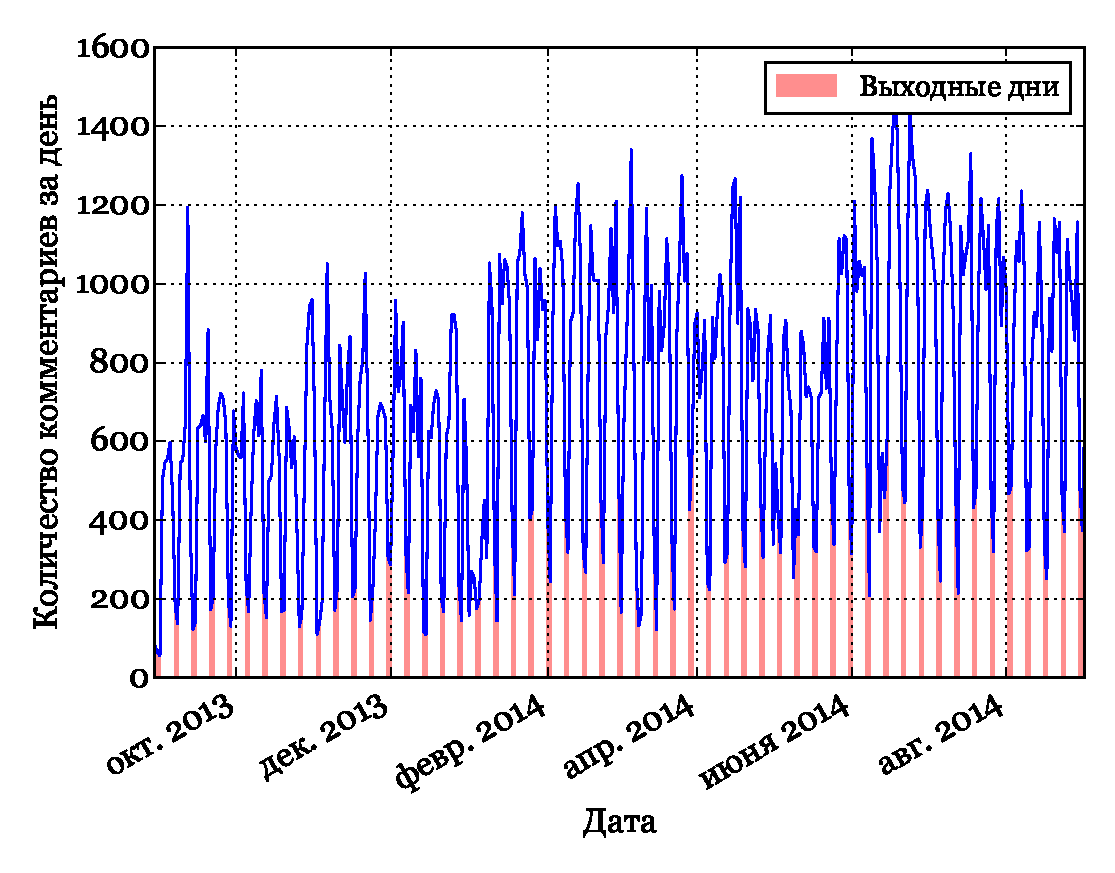
\includegraphics[totalheight=10cm]{comments_by_day}
    \caption{Количество комментариев по дням}
    \label{fig:comments_by_day}
\end{figure}

Анализ графика на рисунке \ref{fig:comments_by_day} позволяет сделать несколько выводов. Во-первых, видно, что в к статьям, которые вышли в выходные дни пользователи оставляют намного меньше комментариев, чем к тем, которые опубликованы в будни. Среднее количество комментариев к статьям в выходного дня составляет 293, в то время как к статьям, написанным в будние дни -- 867.

\section{Комментируемость тем}
\begin{longtable}[c]{|l|c|c|}
	\caption{Самые комментируемые темы}\label{table:comments_by_topics} 
	\\ 
	\hline
	%\multicolumn{3}{|c|}{\textbf{Файл puma\_namelist}}        \\ \hline
	Порядок & Номер темы & Процент комментируемости от наиболее комментируемой \\ \hline
	\endfirsthead   \hline
	\multicolumn{3}{|c|}{\small\slshape (продолжение)}        \\ \hline
	Порядок & Номер темы & Процент комментируемости от наиболее комментируемой \\ \hline
	\endhead        \hline
	\multicolumn{3}{|r|}{\small\slshape продолжение следует}  \\ \hline
	\endfoot        \hline
	\endlastfoot
		1 & 39 & 100.0\% \\
		2 & 25 & 94.0\% \\
		3 & 13 & 86.8\% \\
		4 & 36 & 79.9\% \\
		5 & 2 & 76.2\% \\
		6 & 48 & 74.9\% \\
		7 & 22 & 70.3\% \\
		8 & 27 & 69.7\% \\
		9 & 47 & 67.3\% \\
		10 & 32 & 65.7\% \\
		11 & 14 & 65.1\% \\
		12 & 37 & 65.0\% \\
		13 & 11 & 61.8\% \\
		14 & 1 & 61.6\% \\
		15 & 23 & 61.0\% \\
		16 & 16 & 58.8\% \\
		17 & 21 & 58.7\% \\
		18 & 15 & 57.9\% \\
		19 & 41 & 57.6\% \\
		20 & 42 & 57.1\% \\
		21 & 35 & 56.0\% \\
		22 & 19 & 55.9\% \\
		23 & 9 & 54.6\% \\
		24 & 5 & 54.3\% \\
		25 & 24 & 54.1\% \\
		26 & 0 & 51.6\% \\
		27 & 17 & 51.0\% \\
		28 & 34 & 49.1\% \\
		29 & 43 & 48.2\% \\
		30 & 46 & 47.9\% \\
		31 & 40 & 46.4\% \\
		32 & 31 & 46.2\% \\
		33 & 7 & 45.9\% \\
		34 & 6 & 44.8\% \\
		35 & 10 & 44.7\% \\
		36 & 30 & 43.3\% \\
		37 & 3 & 42.6\% \\
		38 & 29 & 41.7\% \\
		39 & 33 & 41.3\% \\
		40 & 12 & 40.2\% \\
		41 & 38 & 39.8\% \\
		42 & 44 & 39.6\% \\
		43 & 26 & 39.2\% \\
		44 & 45 & 38.7\% \\
		45 & 20 & 37.0\% \\
		46 & 28 & 37.0\% \\
		47 & 49 & 35.4\% \\
		48 & 4 & 34.6\% \\
		49 & 8 & 34.2\% \\
		50 & 18 & 20.7\% \\
	\hline
\end{longtable}
\section{Тональность комментариев по темам}